% !TEX root = morphkasten.tex

\section{Lenkung}


%############## Trapez
\subsection{Trapez}

\begin{figure} [hbp]
	\centering
	\begin{subfigure}[b]{0.4\textwidth}
		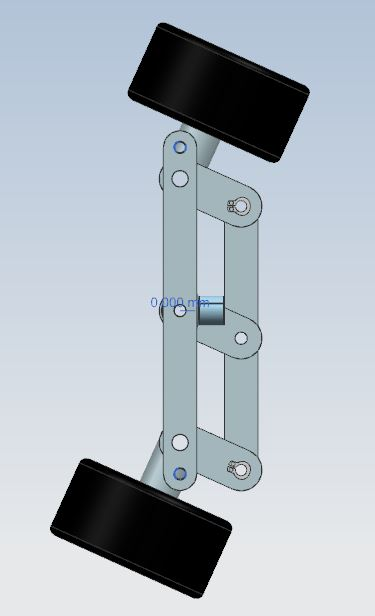
\includegraphics[width=\textwidth]{fig/Trapezlenkung3.JPG}
		\caption{1.Situation: CAD-Modell}
	\end{subfigure}
	\hfill
	\begin{subfigure}[b]{0.36\textwidth}
		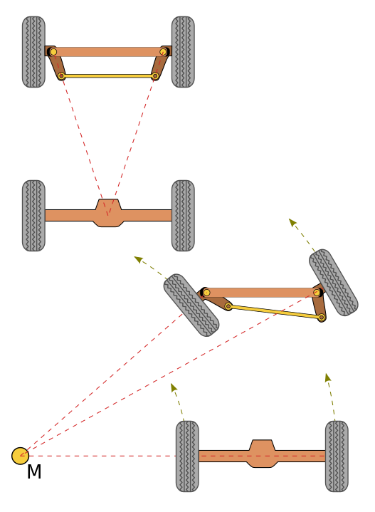
\includegraphics[width=\textwidth]{fig/Lenktrapez.png}
		\caption{2. Situation: Trapezlenkung
		(Quelle: http://www.portmanns.ch/Repetition/Fahrwerk/Lenkungsarten.pdf)}
\end{subfigure}
	\caption{Trapezlenkung}\label{fig:animals}
\end{figure}

\begin{table}[h]
\begin{tabular}{p{0.5\textwidth} | p{0.5\textwidth}}


 \textbf{Vorteile} & \textbf{Nachteile} \\ \hline
	 
\begin{itemize}
\item Konventionelle oft verwendete Lenkung für PWS
\item Berechnungen für Lenkgeometrie im Internet
\item Viele Reale Beispiele als Vorlag
\item ...
\end{itemize}

 
 &
 
\begin{itemize}
\item Herstellung relativ aufwändig
\item Kamera ist in der Kurve nicht 90 Grad zur Strecke
\item Nachteil 3
\item 
\end{itemize}

\end{tabular}
\end{table}

\begin{table}[h]
\begin{tabular}{p{0.5\textwidth}p{0.5\textwidth}}


 \textbf{Risiken} & \\ \hline
	 
\begin{itemize}
\item Bei der Lenkung mit einem Lenktrapez, ist die Kamera in der Kurve nicht 90 Grad zur Fahrbahn. Dies könnte Probleme bei der Bildverarbeitung gegen.
\item Da nur die Vorderachse lenkbar ist, werden die Hinterräder nachgezogen. Dies könnte zu ungenau sein um einen dein Abstand zum Trottoir in einer gewissen Toleranz einzuhalten.
\end{itemize}
&
\begin{itemize}

\end{itemize}

 
\end{tabular}
\end{table}

\pagebreak


%############## Raupen
\subsection{Raupen}
Im Kapitel 1.1 wurden die Variante Raupen bereits beschrieben.


%############## 2 Räder mit 2 Motoren
\subsection{2 Räder mit 2 Motoren}

\begin{figure} [hbp]
	\centering
	\begin{subfigure}[b]{0.36\textwidth}
		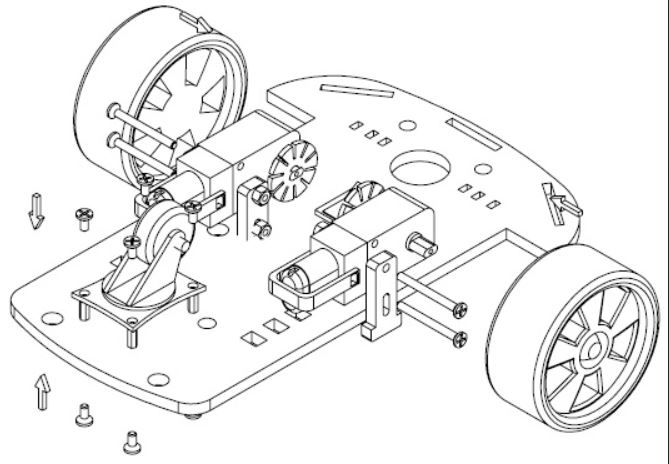
\includegraphics[width=\textwidth]{fig/3rad-3.JPG}
		\caption{2. Situation: Technische Zeichnung
		(Quelle: www.sainsmart.com)}
\end{subfigure}
	\caption{3-Rad Modell}\label{fig:animals}
\end{figure}


\begin{table}[h]
\begin{tabular}{p{0.5\textwidth} | p{0.5\textwidth}}


 \textbf{Vorteile} & \textbf{Nachteile} \\ \hline
	 
\begin{itemize}
\item Selbe Motoren für Antrieb und Lenkung
\item Vorwissen für die Regelung und Ansteuerung MC-Modul an der HSLU
\item Wendekreis sehr klein
\item Kamera ist immer 90 Grad zur Strecke
\end{itemize}

 
 &
 
\begin{itemize}
\item Motoren müssen sehr genau sein
\item Stabilität
\item Keine klare Trennung zwischen Antrieb und Lenkung
\item Regelung schwierig
\end{itemize}

\end{tabular}
\end{table}

\begin{table}[h]
\begin{tabular}{p{0.5\textwidth}p{0.5\textwidth}}


 \textbf{Risiken} & \\ \hline
	 
\begin{itemize}
\item Risiko 1
\item Risiko 2
\end{itemize}
&
\begin{itemize}
\item Risiko 3
\item ...
\end{itemize}

 
\end{tabular}
\end{table}

\pagebreak